\section{效率修正}
当金-金对撞发生时产生双电子对经过或者击中探测器之后被我们测量到,这也就是说我们实际测量到的双电子谱原初信号和最开始产生的双电子谱相比是有探测器的接收度和效率损失的。在实验上,如果说两个结果要进行比较,这两个结果应该是一个对等的比较,即两者的结果应该是在相同的条件下得到的结果。对于STAR探测器来说,在使用的子探测器相同且结构固定的情况下,所有STAR的测量结果是在同一个接收度下的结果。而在同一个接收度(STAR接收度)下,在不同年份不同的能量下探测器的效率也会有差异。所以在和STAR的其他测量进行比较时,我们需要对原初信号进行效率修正,从而得到在STAR接收度下的双电子谱。
对于本分析而言,得到在STAR接收度下的双电子谱需要对原初信号进行如下修正:
\begin{equation}
    N_{STAR~acc.} = \frac{ N_{raw~signal} }{ \epsilon_{pair~eff.} }
\end{equation}
\begin{equation}
    \epsilon_{pair~eff.} = \epsilon_{e^{+}}\times\epsilon_{e^{-}}
\end{equation}
\begin{equation}
    \label{eq:single_e}
    \epsilon_{e} = \epsilon_{TPC}\times\epsilon_{TOF}\times\epsilon_{eID}
\end{equation}
其中$\epsilon_{pair~eff.}$为电子对探测效率,其为 \eplus 与 \eminus 的效率乘积。$\epsilon_{TPC}$, $\epsilon_{TOF}$和$\epsilon_{eID}$分别为TPC径迹重建效率,TOF探测效率,以及电子鉴别效率。这几项将会在接下来的几个小节当中分别讨论。

\subsection{TPC径迹重建效率}
当粒子穿过TPC的时候,需要在TPC中留下足够多的点来进行径迹重建和计算 $\langle dE/dx \rangle$, 这就对径迹的质量有了要求,从而带来了效率损失。
计算TPC径迹探测效率的公式如下:
\begin{equation}
    \epsilon_{TPC} = \frac{ nTrack( N_{HitsFit} \geq 20~\&\&~\frac{N_{HitsFit}}{N_{HitsPoss}}~\&\&~N_{HitsPoss}\geq15~\&\&~dca\leq1~\&\&~|\eta| < 1 ) }{nTrack(|\eta| < 1)}
\end{equation}

因为我们无法知道粒子在被时间投影室探测到之前的状态,我们只能通过模拟的方式来计算时间投影室的径迹重建效率。在STAR实验中,这种模拟的方式被称作embedding。将蒙特卡洛(Monte Carlo)模拟得到的径迹信息在进行径迹重建之前和实际数据混合在一起后再用时间投影室进行径迹重建。从而可以得到时间投影室重建之前和之后的径迹的数量比。在这个过程中,所有的模拟径迹会被随机分配到所有的run当中,每个run中混入的模拟径迹数占总径迹数的百分比固定,以期能更好地反应整个取数过程中时间投影室的平均效率。又因为探测器本身接收度的问题,在不同的 \pt , $\eta$, $\phi$区间不能对效率进行简单的平均。例如在时间投影室扇区和扇区之间的支撑结构对应$\phi$区间,会因为支撑结构带来的死区导致效率下降。如果在计算效率时使用的$\phi$区间过大,将导致此位置的效率被平均,无法正确反应整个时间投影室的探测效率。所以我们将整个模拟数据根据 $\eta$, $\phi$,分为了 10 $\times$ 36个区间,在每个区间计算随 \pt 变化的效率。图\ref{fig:TPCTracking} 展示了在不同中心度下时间投影室的径迹重建效率。

\begin{figure}[htb]
    \begin{center}
    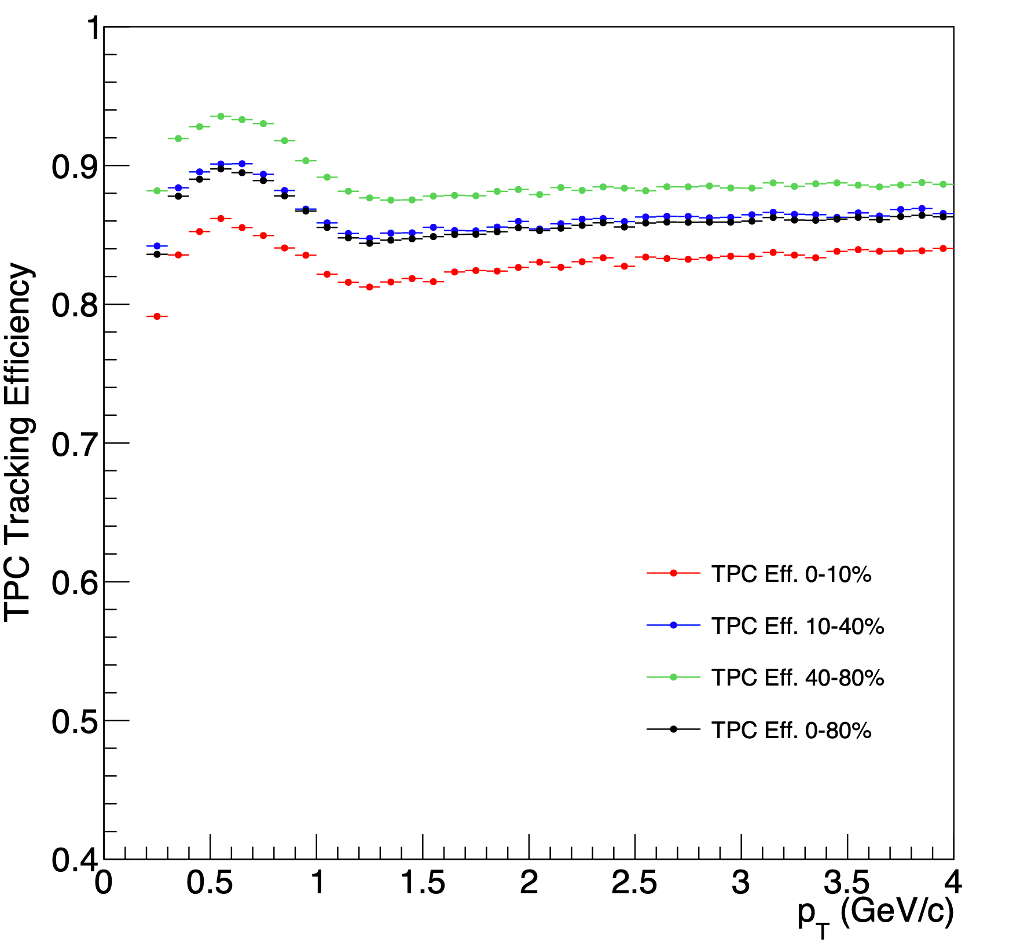
\includegraphics[width=0.75\textwidth,clip]{figures/Chapter4/TPCTracking.png}
    \end{center}
    \caption[不同中心度下时间投影室径迹重建效率示意图]{不同中心度下时间投影室径迹重建效率示意图,不同颜色的点为不同中心度下的径迹重建效率,图中所示效率为对所有$\eta$, $\phi$区间积分后的效率}
    \label{fig:TPCTracking}
\end{figure}

\subsection{TOF探测效率}
因为粒子在穿过时间投影室后再击中飞行时间探测器,所以飞行时间探测器的匹配效率可以直接分析数据得到。计算TOF探测效率的公式如下:
\begin{equation}
    \epsilon_{TOF} = \frac{ nTracks(TOF~Matched) }{ nTracks(TPC) }
\end{equation}
其中nTracks(TOF Matched)为穿过TPC,通过径迹质量判选并且在TOF上可以找到对应击中的径迹, nTracks(TPC)为TPC探测到的径迹数.为了更好的反应接收度对效率的影响,和TPC探测效率类似,所有数据根据 $\eta$, $\phi$,分为了 10 $\times$ 36个区间,在每个区间计算随 \pt 变化的效率。但因为在每个事例中产生的电子数量较少,直接用电子来计算TOF探测效率的话统计过低,无法很好的估计TOF探测效率。所以在本分析中,我们先用 \piplus 和 \piminus 来计算三维( \pt , $\eta$, $\phi$ )的TOF探测效率,并计算随着 \pt 变化的$\pi$介子和电子效率比值用来修正$\pi$介子和电子效率之间的差异。

\begin{figure}[htb]
    \centering
    \begin{subfigure}[b]{0.47\textwidth}
        \centering
        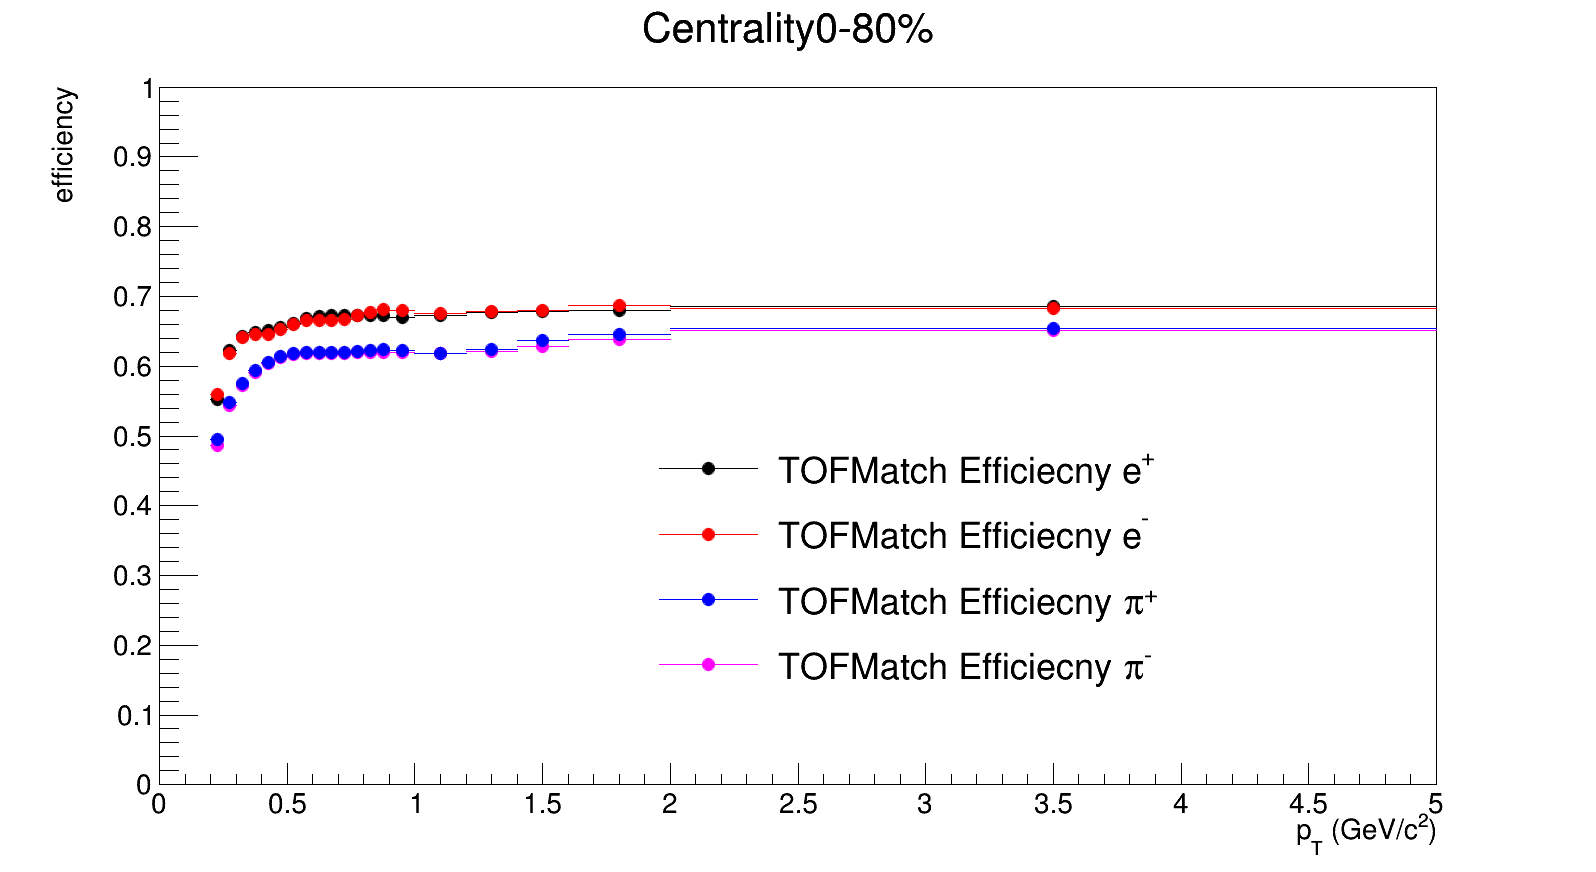
\includegraphics[width=\textwidth,clip]{figures/Chapter4/Eff_Centrality080.png}
        \caption{}
        \label{fig:TOF_match_eff}
    \end{subfigure}
    \hfill
    \begin{subfigure}[b]{0.47\textwidth}
        \centering
        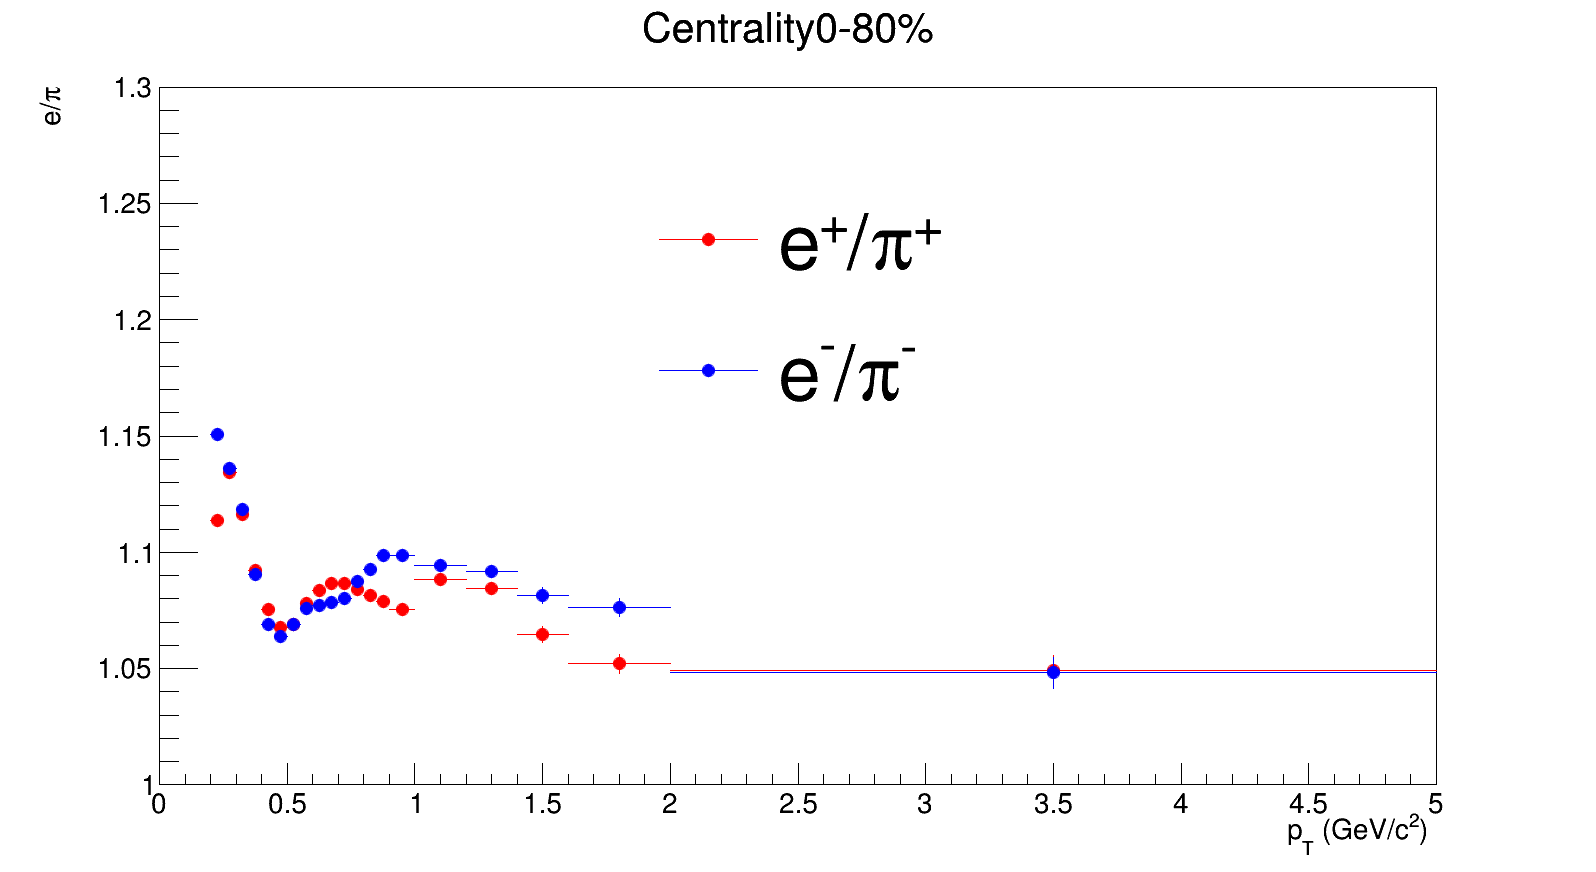
\includegraphics[width=\textwidth,clip]{figures/Chapter4/Ratio_Centrality080.png}
        \caption{}
        \label{fig:pi_e_ratio}
    \end{subfigure}
       \caption[飞行时间探测器匹配效率]{图\ref{fig:TOF_match_eff}为0-80\%中心度下正负电子和正负$\pi$介子的飞行时间探测器匹配效率。图\ref{fig:pi_e_ratio}为正负电子和正负$\pi$介子的效率差别}
       \label{fig:TOFEff}
\end{figure}

\subsection{电子鉴别效率}

在STAR的分析当中我们是采用TPC测量的dE/dx(${\rm n\sigma_e}$)和TOF测量的速度($1/\beta$)信息来进行粒子鉴别,在 \ref{ch:eID} 一节当中已经进行过介绍,理想情况下两者应该分别为中心值为0和1的高斯分布。但因为探测器的原因中心值可能发生偏移,分布也会变宽,这样会有一部分电子落在电子鉴别的判选条件范围之外导致效率损失。要计算电子鉴别判选带来的效率损失,首先要获得一个纯的电子数据样本。在本分析当中,纯电子的数据样本通过筛选电子对质量的方式选出。如图\ref{fig:PureElectron}所示。在极低的电子对质量区间,电子对的来源主要是光子转换产生的电子。在这个区间有着电子纯度高,背景少的优点,所以我们选取对质量${\rm M_{ee} < 0.015~GeV}$质量区间内的电子作为我们的纯电子sample。对于 \nSigmaE 的判选条件,在计算电子纯度的时候时候一并被计算出来,如图{\color{red} 示意图}所示,其中拟合的一倍$\sigma$置信区间被用来作为系统误差。对于$1/\beta$的判选条件,在得到纯电子样本之后通过拟合和bin counting两种方式计算得到效率,这两种效率之间的差别被用作系统误差。

\begin{figure}[htb]
    \begin{center}
    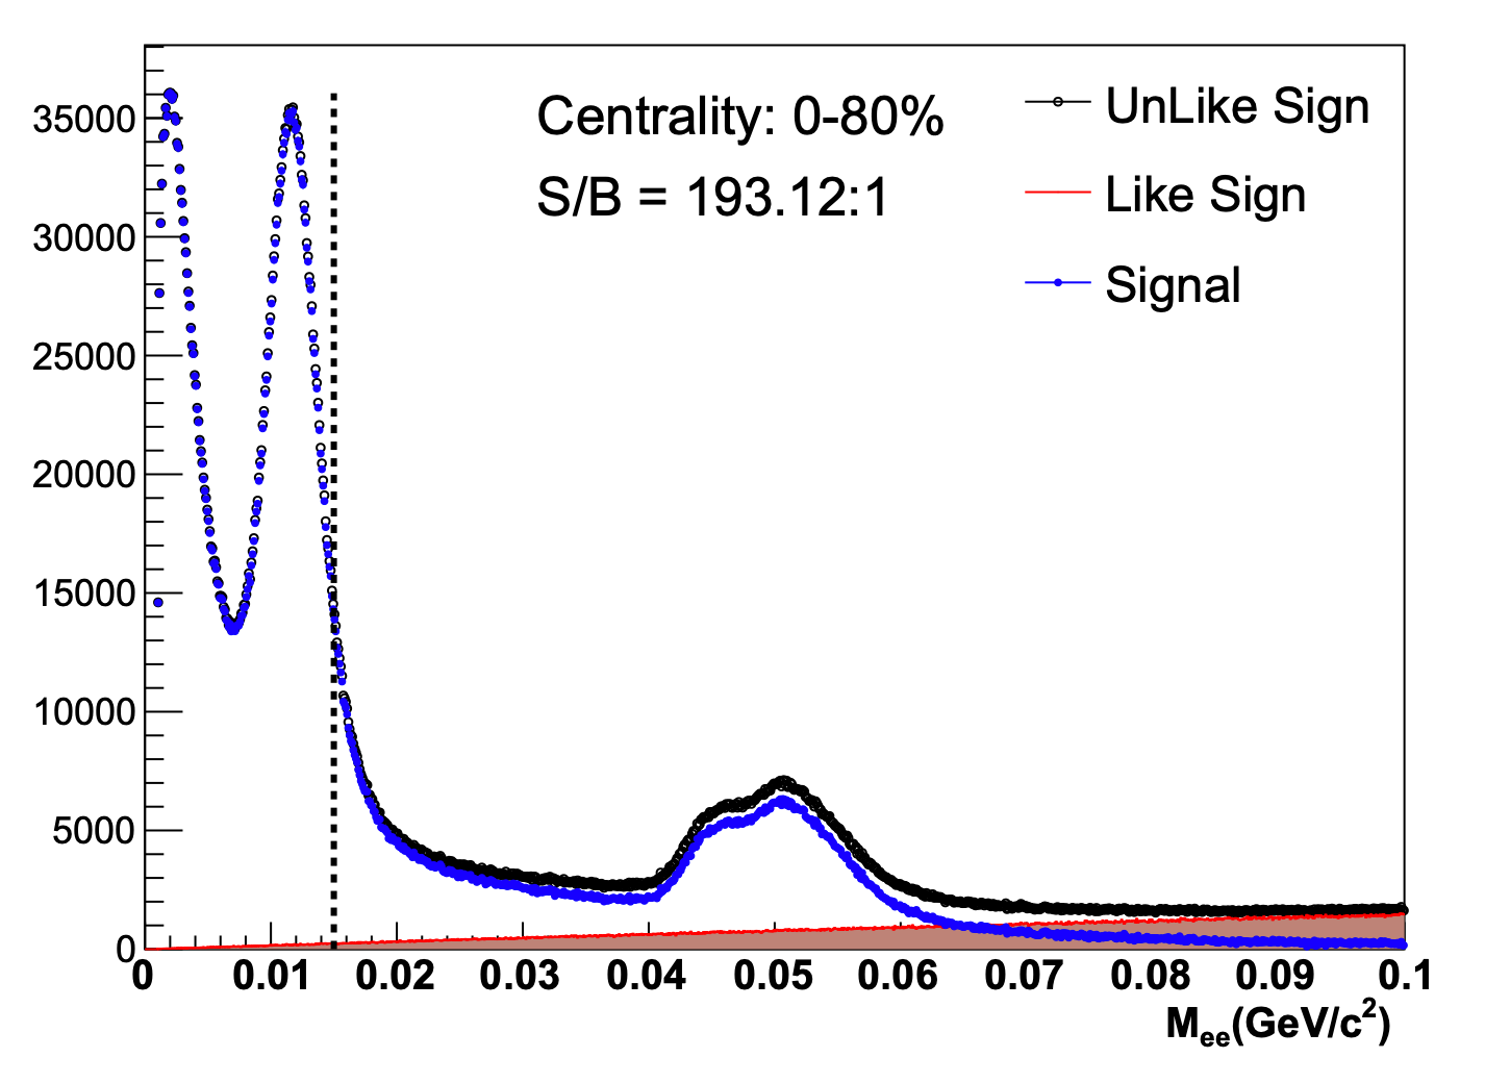
\includegraphics[width=0.75\textwidth,clip]{figures/Chapter4/PureElectron.png}
    \end{center}
    \caption[纯电子数据样本选择范围]{纯电子样本选择示意图。在双电子谱当中,极低质量区间(${\rm M_{ee} < 0.015~GeV}$)的信噪比可以达到193:1,被选作纯电子样本的选择区间}
    \label{fig:PureElectron}
\end{figure}

\begin{figure}[htb]
    \centering
    \begin{subfigure}[b]{0.47\textwidth}
        \centering
        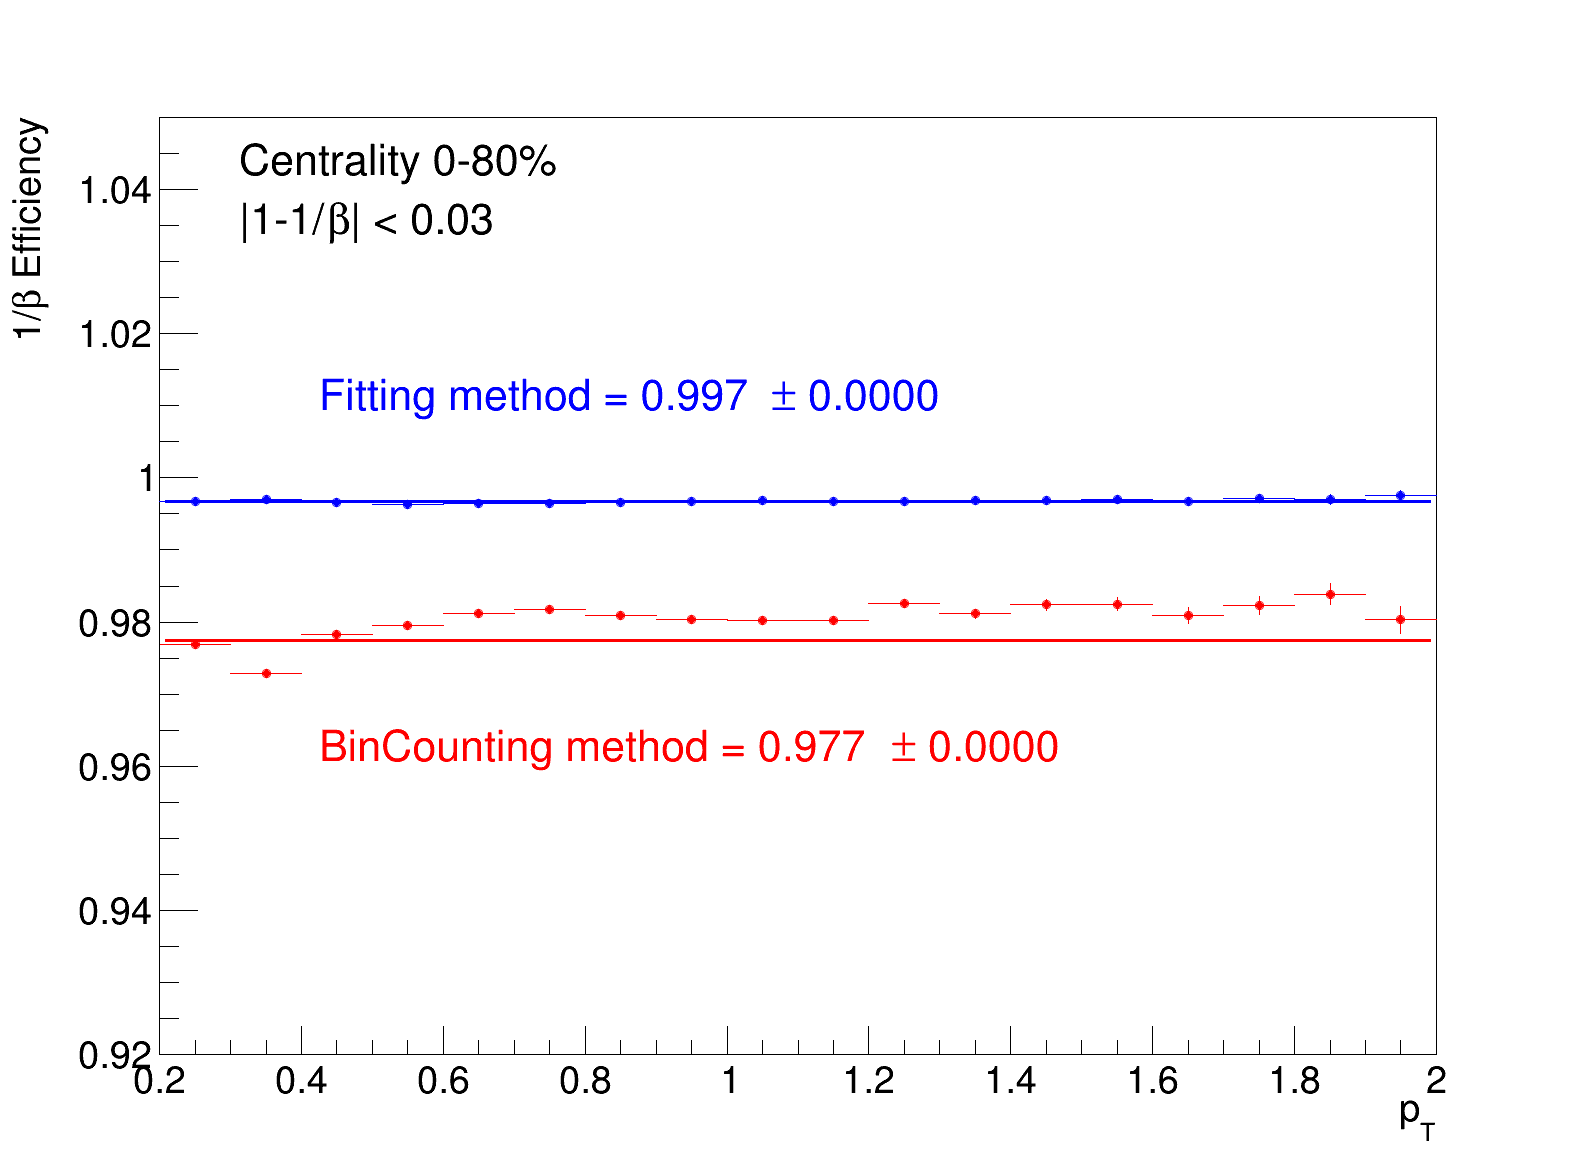
\includegraphics[width=\textwidth,clip]{figures/Chapter4/beta_cut_eff_080.png}
        \caption{}
        \label{fig:beta_cut_eff_080}
    \end{subfigure}
    \hfill
    \begin{subfigure}[b]{0.47\textwidth}
        \centering
        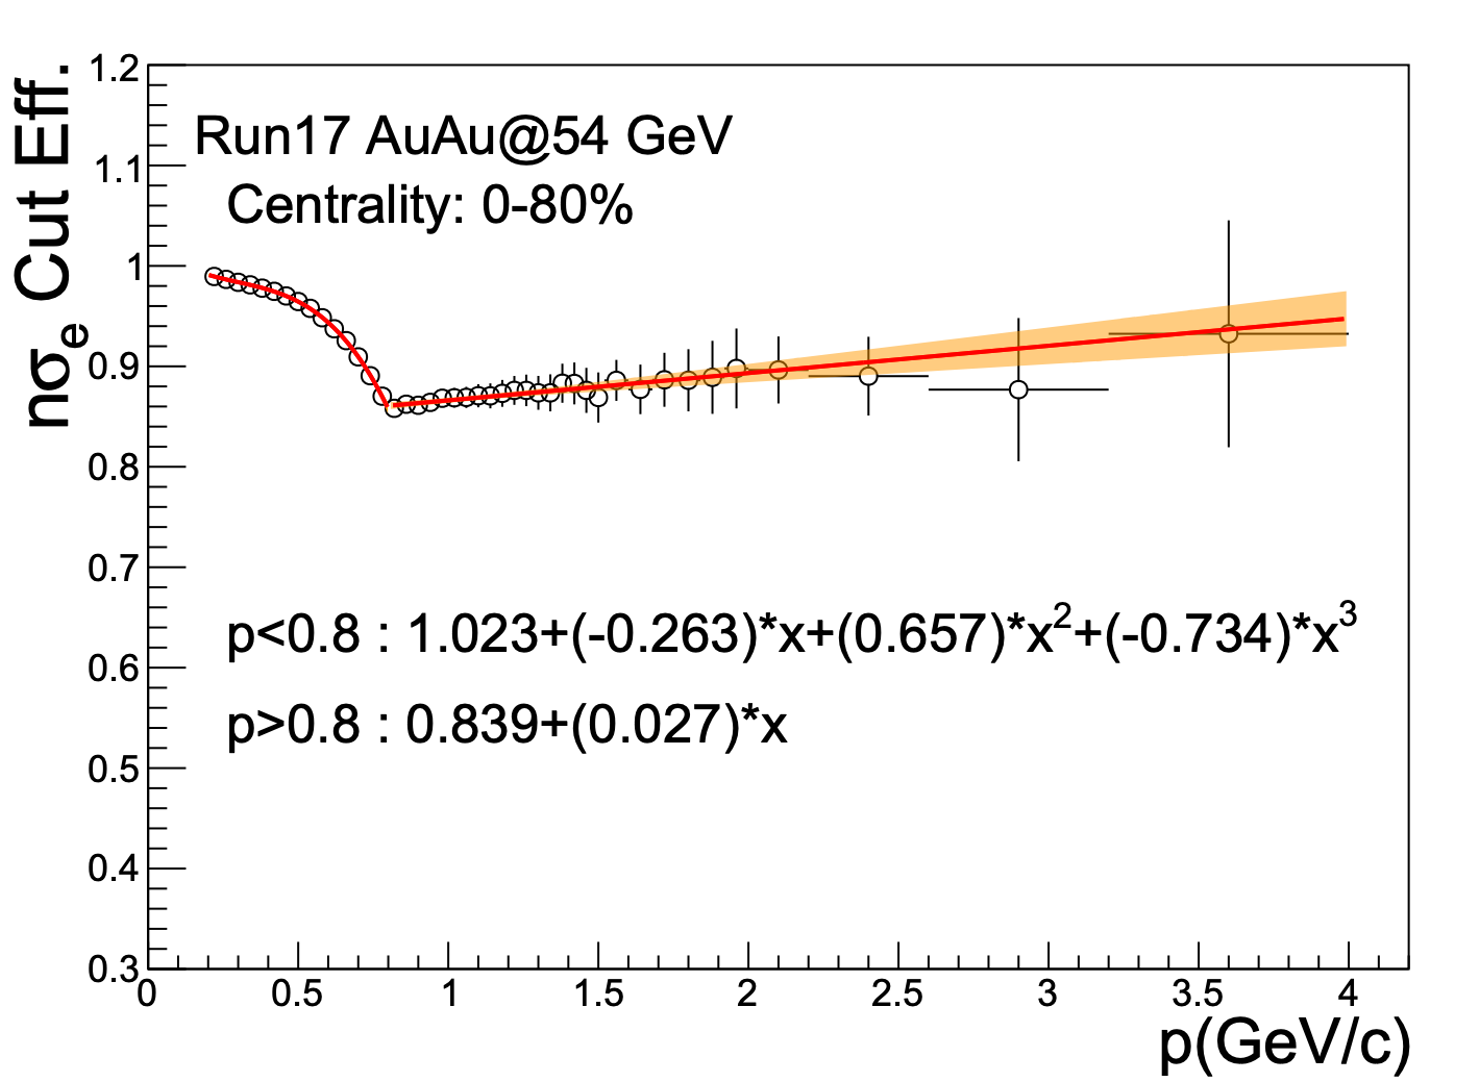
\includegraphics[width=\textwidth,clip]{figures/Chapter4/nSigmaE_cut_eff.png}
        \caption{}
        \label{fig:nSigmaE_cut_eff}
    \end{subfigure}
       \caption[电子鉴别效率示意图]{图\ref{fig:beta_cut_eff_080}为0-80\%中心度下1/$\beta$的电子鉴别效率,其中两种不同的方法计算的效率的误差。图\ref{fig:pi_e_ratio}为正负电子和正负$\pi$介子的效率差别}
       \label{fig:TOFEff}
\end{figure}

\subsection{双电子效率修正}
\label{chap:pair_eff}

因为最后我们是得到的双电子谱,所以在最后进行效率修正的时候我们需要的是双电子对的重建效率。在本分析当中,电子对在二维空间($p_T~-~M_{ee}$平面)上重建效率是通过蒙特卡洛模拟(Monte Carlo Simulation)的方法计算得到的。而对于双电子的来源,我们有两种不同的模拟方法:
\begin{itemize}
    \item[1.]虚光子模拟:在这种方法中由虚光子对作为整个模拟的输入。对于虚光子来说,其动力学性质如下:在强子衰变模拟(将于\ref{ch:cocktail}讨论)当中得到的$p_T$和$M_{ee}$的来作为其$p_T$和$M_{ee}$的输入分布。其方位角$\phi$和快度(rapidity)分布分别为在$-\pi~-~\pi$以及-1 - 1范围内的平的分布。同时在虚光子在整个空间各向同性地衰变为双电子对。
    \item[2.]强子衰变模拟:在这种情况下的双电子分布为来自于已知的各种来源的混合。强子的衰变在模拟时所用的方法和虚光子模拟类似,也是在整个空间各向同性的衰变为双电子对,但是对于来源于重味强子的半轻子衰变的双电子,其由Pythia模拟产生,在这个过程中产生的双电子对是强相关的。
\end{itemize}
单电子的探测效率通过式\ref{eq:single_e}计算得到。对于电子对来说,每一个电子能否被探测器重建出来都是一个独立的事件,所以电子对的重建效率为两个电子探测效率的乘积,即$\epsilon_{pair} = \epsilon_{e^+}~*~\epsilon_{e^-}$。单电子在进行pT smearing之后再组合成电子对,并在添加电子对探测效率的权重修正之后填入$p_T~-~M_{ee}$的二维直方图。在STAR的接收度($p_T^{e} > 0.2~{\rm GeV/c}$, $|Y_{ee} < 1|$ 以及 $|\eta_e| < 1$)内,如式通过计算添加效率权重修正和未添加效率权重两个直方图之间的比值得到在不同区间内的双电子探测效率。图\ref{fig:Compare_PairEff}为\sNN = 54.4 GeV金-金对撞当中不同中心度下的双电子重建效率。

\begin{figure}[htb]
    \begin{center}
    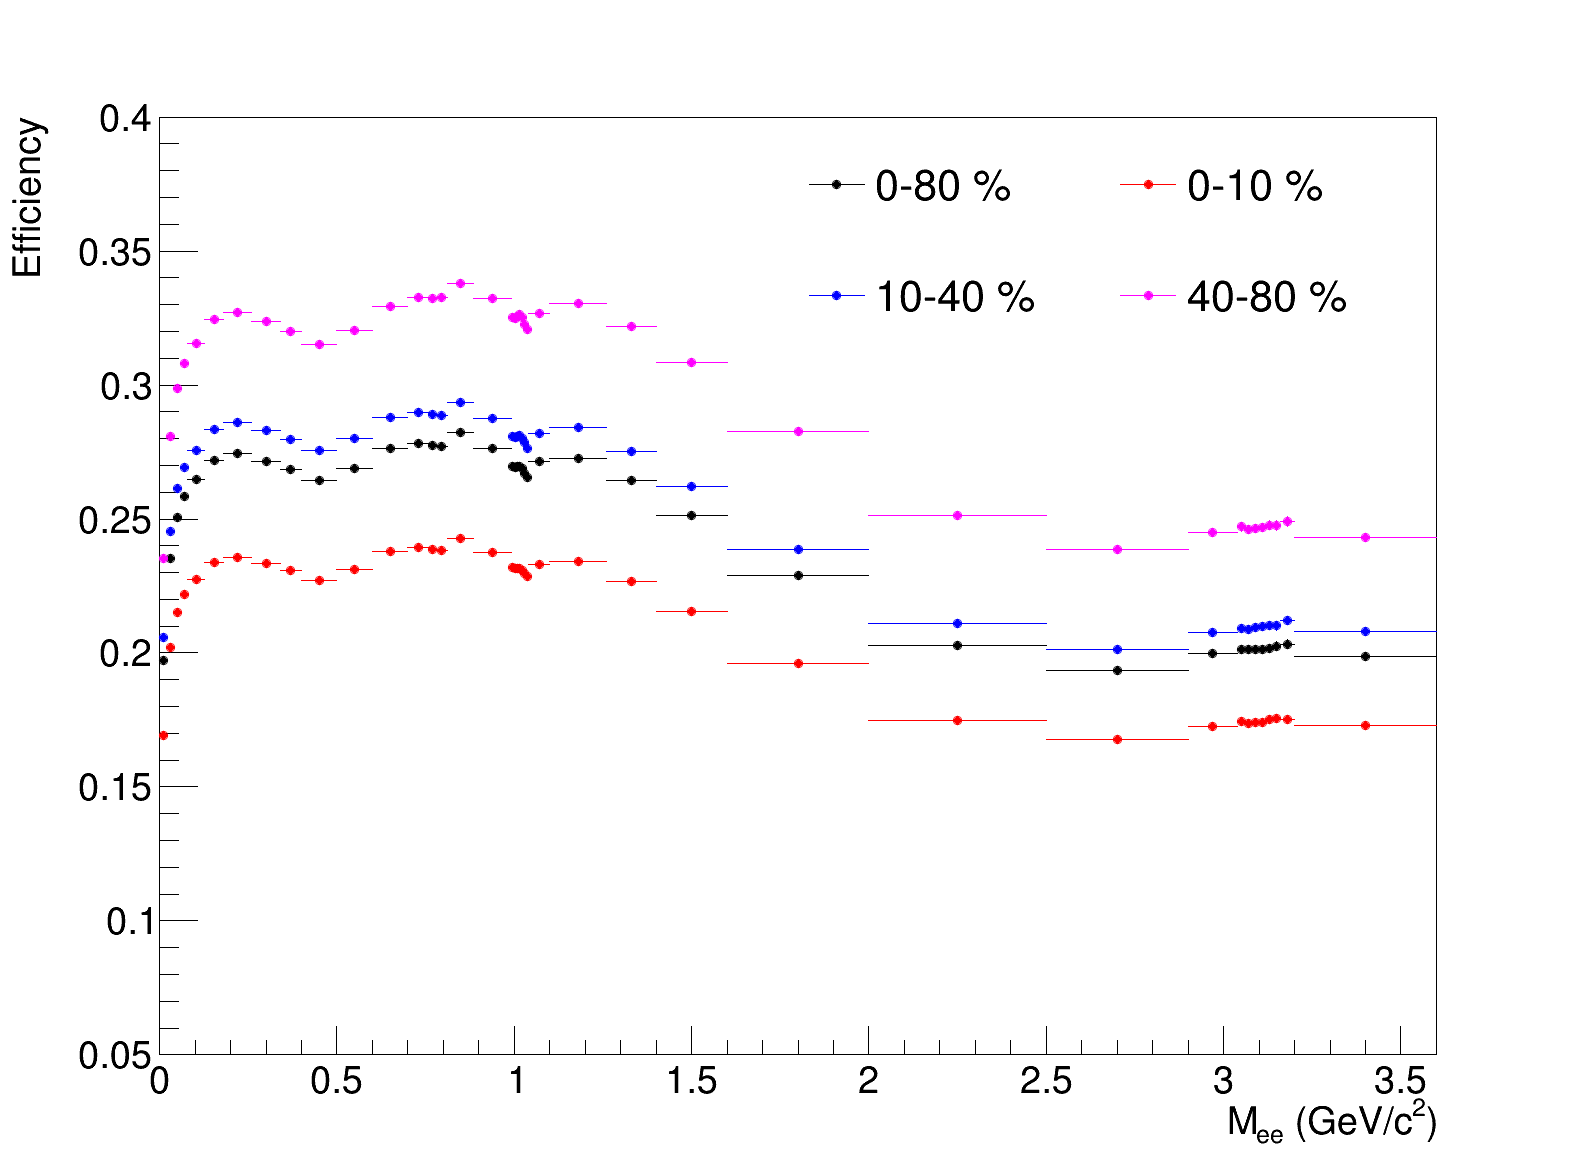
\includegraphics[width=0.75\textwidth,clip]{figures/Chapter4/Compare_PairEff.png}
    \end{center}
    \caption[不同中心度下的双电子重建效率]{\sNN = 54.4 GeV金-金对撞当中不同中心度下的双电子重建效率}
    \label{fig:Compare_PairEff}
\end{figure}

\subsection{接收度修正}
\label{chap:pair_acc}

在上一小节当中我们提到了STAR的接收度,如果我们要将STAR的测量结果和其他实验当中的结果进行比较,我们需要做的是要将STAR的结果修正到全空间当中去,消除STAR接收度的影响。而STAR的接收度修正因子可以通过和双电子效率类似的方式计算得到。计算方法如式\ref{eq:STAR_acc}所示。图\ref{fig:Accep_VP}\sNN = 54.4 GeV金-金对撞当中通过虚光子作为输入计算得到的STAR接受度修正因子。
\begin{equation}
    \label{eq:STAR_acc}
    f_{STAR acc.} = \frac{nPairs(p_T^{e} > 0.2~{\rm GeV/c} \&\& |Y_{ee} < 1| \&\& |\eta_e| < 1)}{nPairs}
\end{equation}
\begin{figure}[htb]
    \begin{center}
    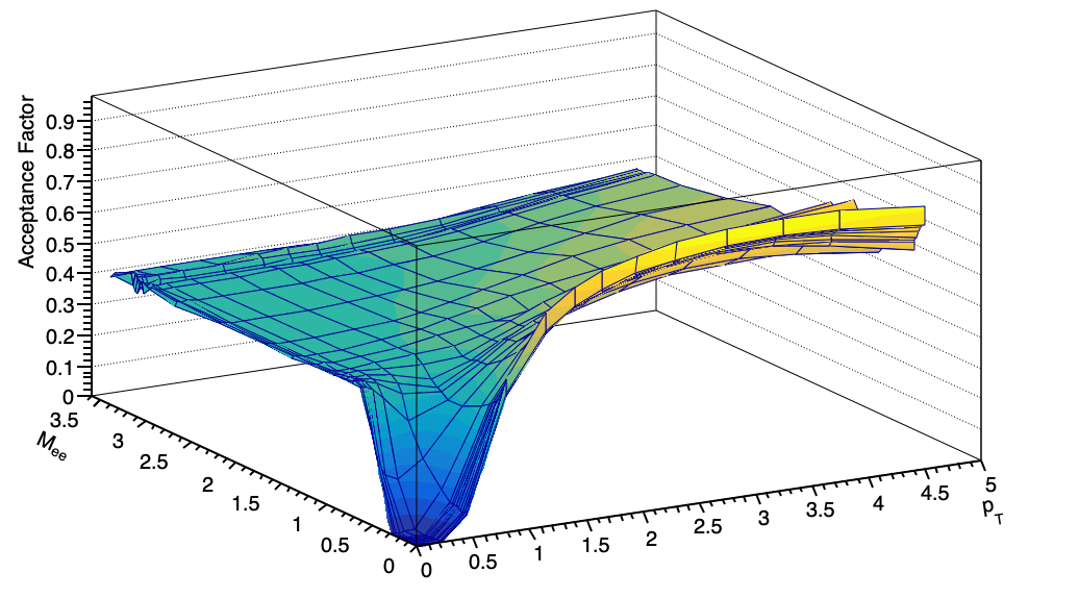
\includegraphics[width=0.75\textwidth,clip]{figures/Chapter4/Accep_VP.png}
    \end{center}
    \caption[通过虚光子作为输入计算得到的STAR接受度修正因子]{\sNN = 54.4 GeV金-金对撞当中通过虚光子作为输入计算得到的STAR接受度修正因子}
    \label{fig:Accep_VP}
\end{figure}
